\chapter{Motivating Scenario}
\label{chap:motivatingScenario}

In order to realize the Organizational Modeling, the below motivating scenario has been taken and realized using the developed UI editor.
This scenario also helps in testing the UI editor along with realizing the Organizational Notations. The motivating scenario has been chosen based on the advice provided in works ..... The figure of this example was taken from the context of manufacturing sector. The  intention of the organization is to increase the quarterly revenue and number of unit sales. In order to achieve this intention through Organizational Modeling Approach, as a first step we need to break the abstract intention into several strategies like
\begin{enumerate}
	\item Increasing the revenue through expanding the market sales. 
	\item Through improving the excellence of the product which in turn brings back old and new customers.
	\item Through increasing the advertisement which helps in customer knowing about the product.
\end{enumerate}

%%%%%%%%%%%%%%%%%%%%%%%%%%%%%%%%%%%%%%%%%%%%%%%%%%%%%%%%%%%%%%%%%%%%%%%%%
\section{Overview}
\label{sec:overview}
%%%%%%%%%%%%%%%%%%%%%%%%%%%%%%%%%%%%%%%%%%%%%%%%%%%%%%%%%%%%%%%%%%%%%%%%%
-- An abstract overview about how collaborations take place inside any organizations---
 





%%%%%%%%%%%%%%%%%%%%%%%%%%%%%%%%%%%%%%%%%%%%%%%%%%%%%%%%%%%%%%%%%%%%%%%%%
\section{Resource-centric Organizational Modeling Example}
%%%%%%%%%%%%%%%%%%%%%%%%%%%%%%%%%%%%%%%%%%%%%%%%%%%%%%%%%%%%%%%%%%%%%%%%%
 The concept of Organizational Model Notations can be explained with the following manufacturing scenario. ABC Ltd. is a budding computer technology company which designs, develops, manufactures and sells personal computers, tablets and laptops. The CEO's goal of the quarter is to increase the revenue and number of unit sales. The initial context describes the situation that motivates to start the process. The final context describes the situation that is achieved once the process completed successfully. Goals connect initial context definitions with final context definitions \cite{Sungur2014a}. The sub-goals are the intermediate goals which describes the expected outcome in a measurable form. Goals are reached through strategy implementation which is plan of action designed to meet a goal. 

 The example scenario ABC Ltd. helps in understanding the organizational modeling i.e., how organization's higher level goal can be achieved by amalgamation of specific, measurable and realistic sub-goals. . The whole view has been divided into Goal view and Strategy view. The \textit{Goal View} shown in the Figure\ref{fig:goalview} provides only the details of goal and its associated strategies. There can be multiple strategies followed to achieve a goal. The \textit{Strategy View} shown in the Figure\ref{fig:strategyview} connects big picture of each strategy with individual goals that has to be carried out. In Organizational Process Modeling, strategies are self-contained and loosely coupled. So that when we extract only the strategies from Organization Process Modeling it would be similar to Informal Process Essential Modeling. 

 The Strategy view  in the Figure\ref{fig:strategyview} depicts big picture of each strategy. Strategies are associated with both goals and capabilities. Capabilities are related to goals and resources. As each goal needs certain capability to successfully execute the goal they both are connected using the verb \textit{"requires"}. Resources are the potential holder of the capability i.e., to satisfy a capability we need resources. The capability and its associated resources are linked using the verb \textit{"satisfied-by"}. 


\begin{figure}
	\centering
	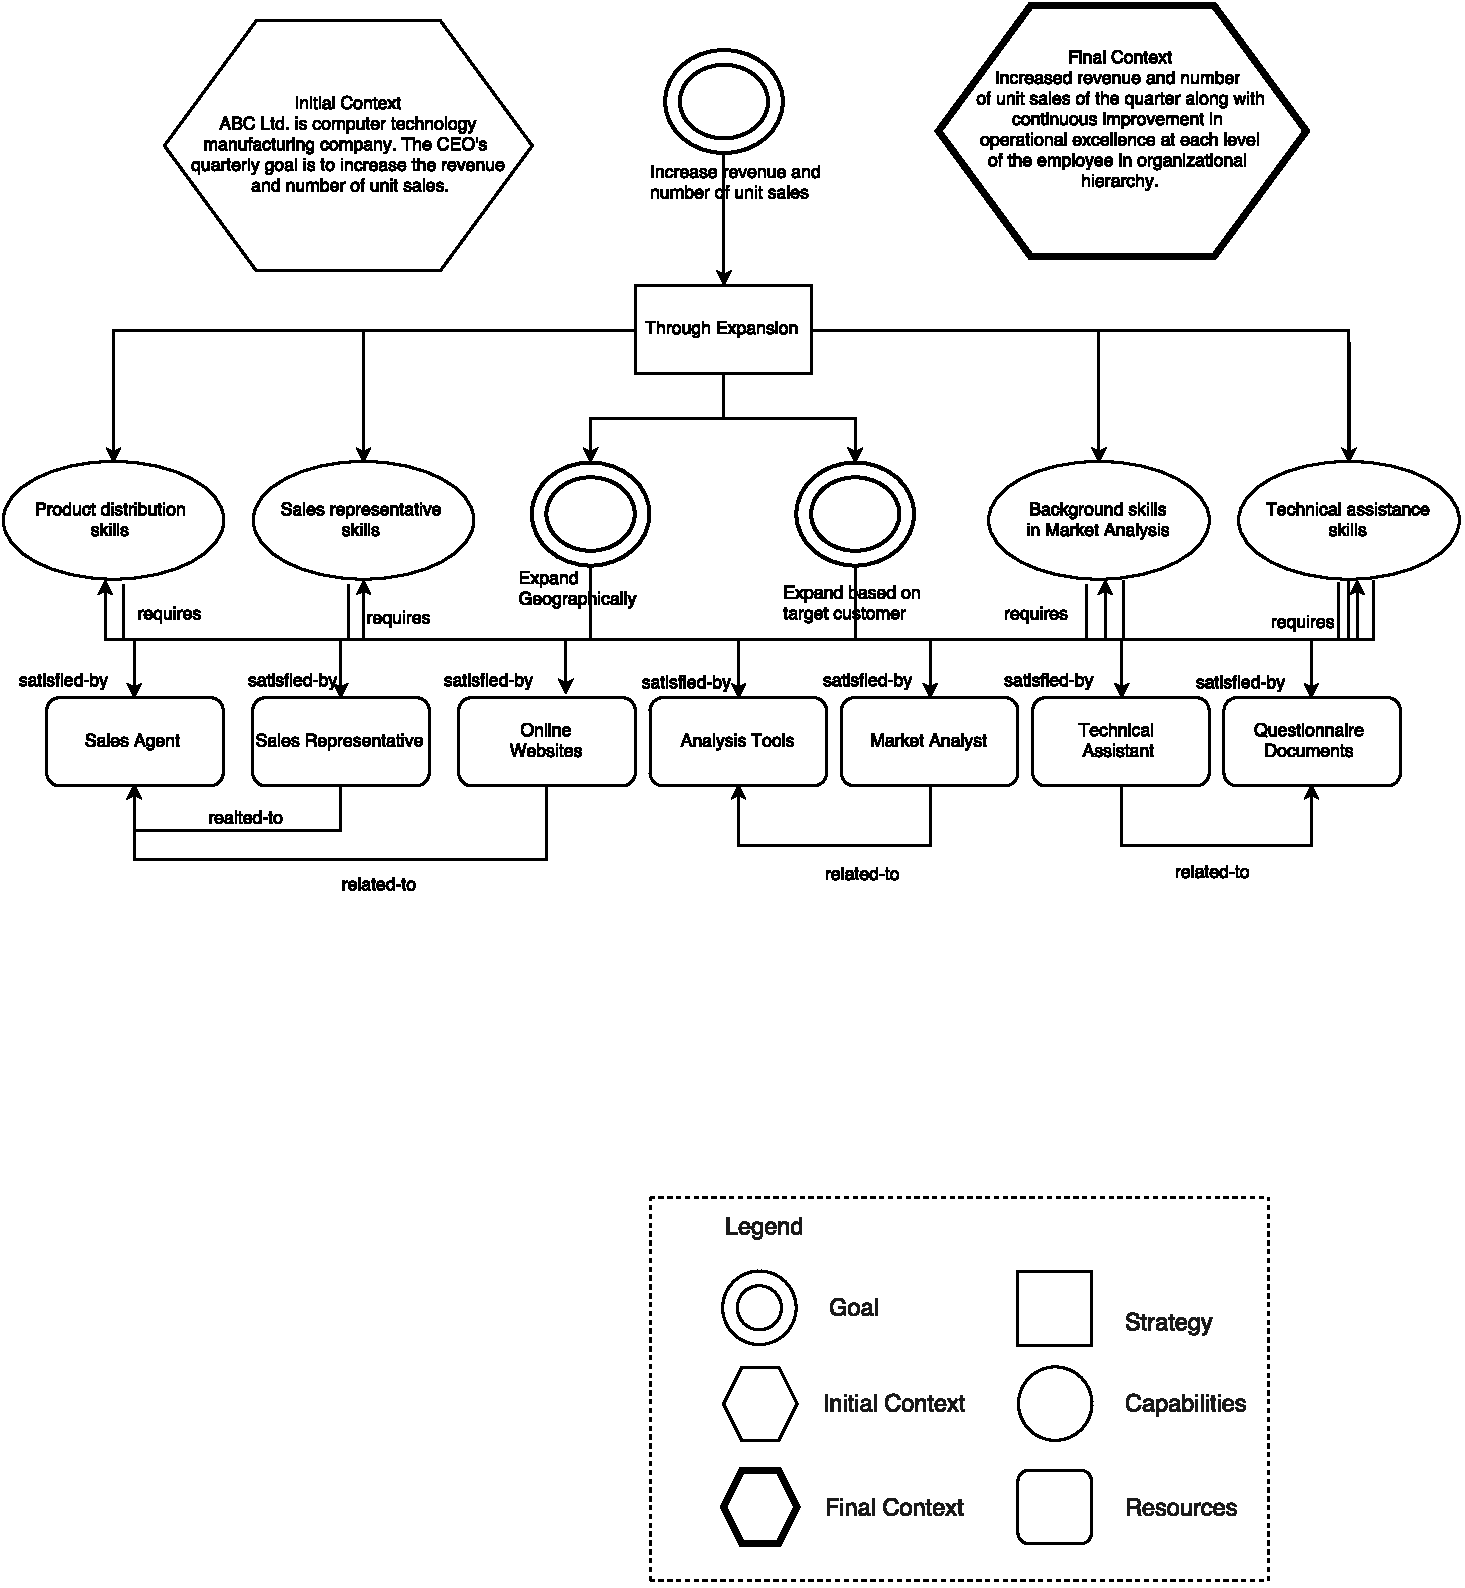
\includegraphics[width=\textwidth]{StrategyView.pdf}
	\caption{Strategy View}
	\label{fig:strategyview}
\end{figure}

\begin{figure}
	\centering
	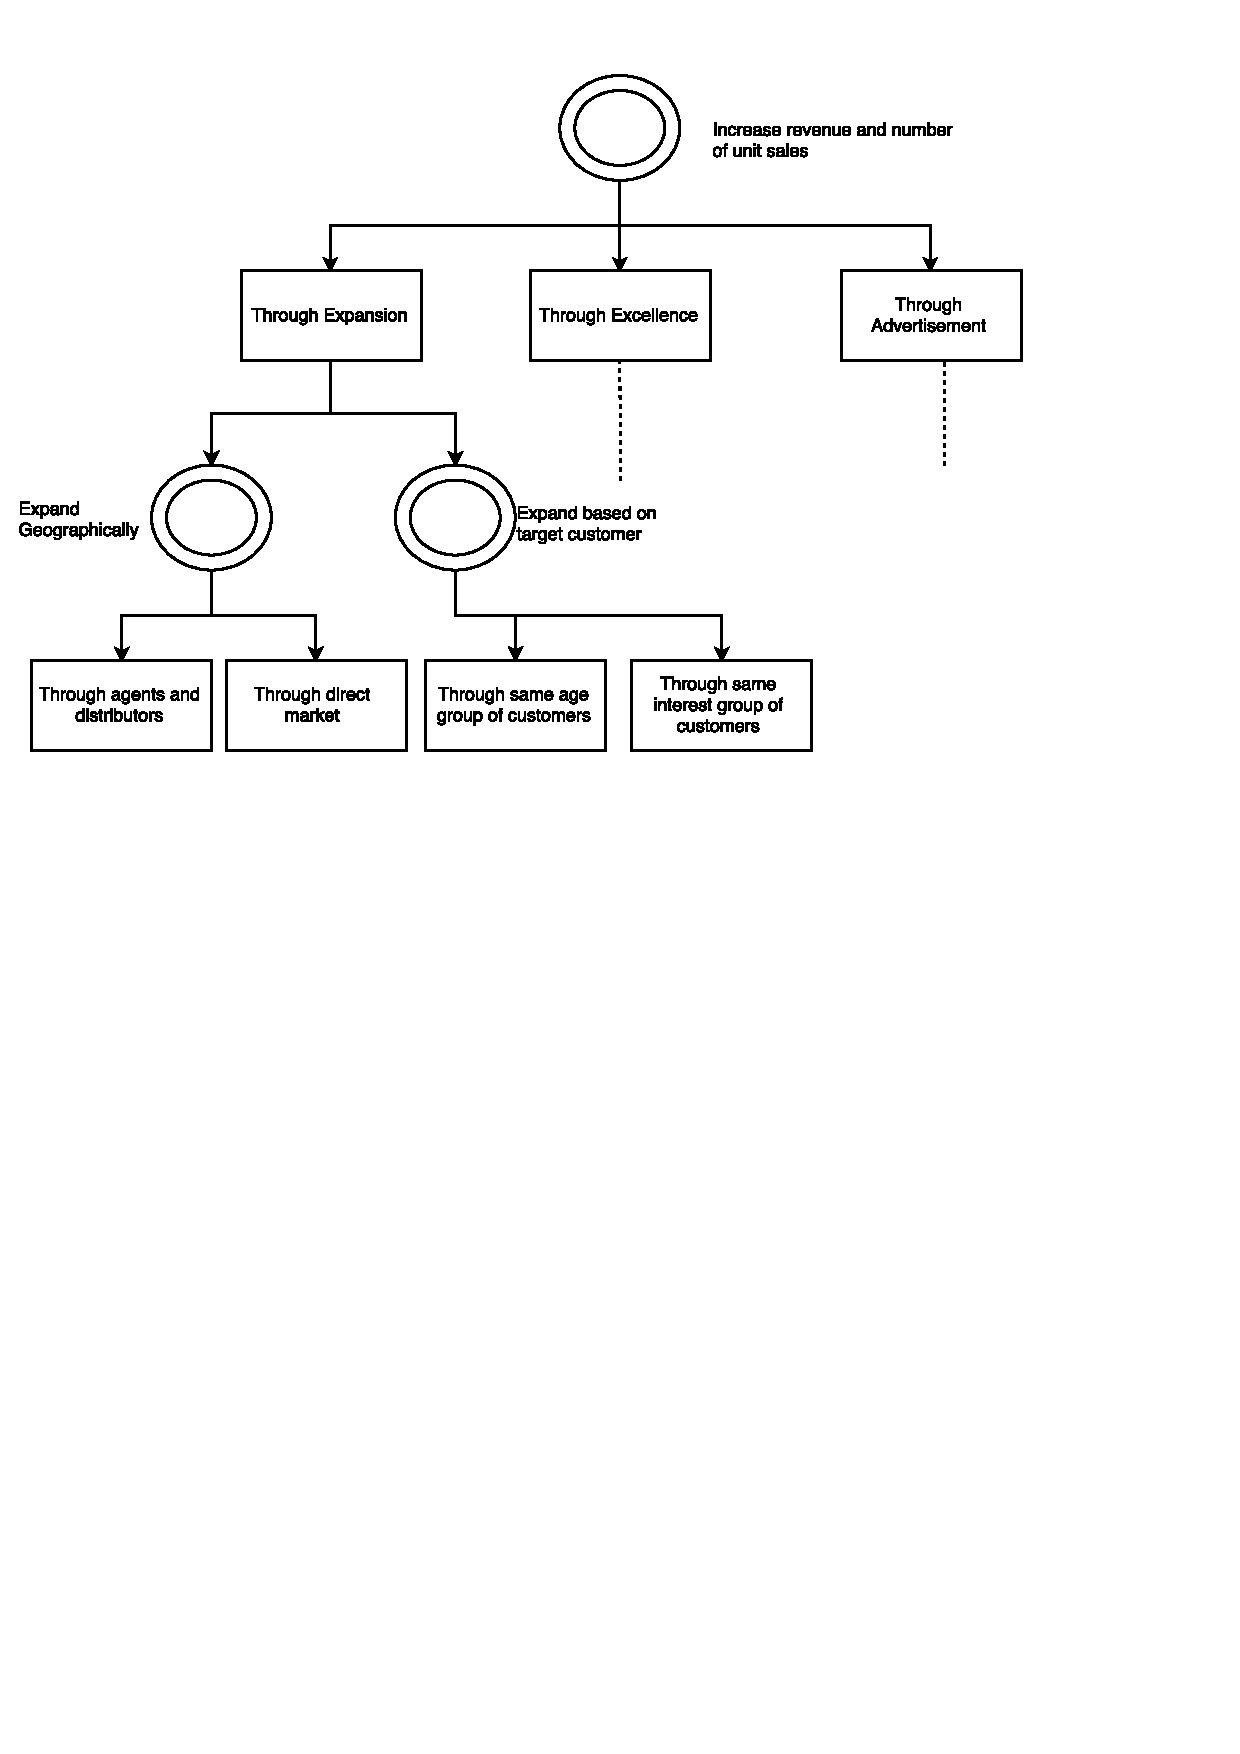
\includegraphics[width=\textwidth]{GoalView.pdf}
	\caption{Goal View}
	\label{fig:goalview}
\end{figure}

%%%%%%%%%%%%%%%%%%%%%%%%%%%%%%%%%%%%%%%%%%%%%%%%%%%%%%%%%%%%%%%%%%%%%%%%%
\section{An Abstract View of Entity Types}
\label{sec:entities}
%%%%%%%%%%%%%%%%%%%%%%%%%%%%%%%%%%%%%%%%%%%%%%%%%%%%%%%%%%%%%%%%%%%%%%%%%
 --- This section discusses in details, about each entity types of the motivating scenario and 
 their images---
 

%%%%%%%%%%%%%%%%%%%%%%%%%%%%%%%%%%%%%%%%%%%%%%%%%%%%%%%%%%%%%%%%%%%%%%%%%
\subsection{Organizational Intentions} 
\label{sec:intentions}
%%%%%%%%%%%%%%%%%%%%%%%%%%%%%%%%%%%%%%%%%%%%%%%%%%%%%%%%%%%%%%%%%%%%%%%%%


%%%%%%%%%%%%%%%%%%%%%%%%%%%%%%%%%%%%%%%%%%%%%%%%%%%%%%%%%%%%%%%%%%%%%%%%%
\subsection{Organizational Strategies} 
\label{sec:strategies}
%%%%%%%%%%%%%%%%%%%%%%%%%%%%%%%%%%%%%%%%%%%%%%%%%%%%%%%%%%%%%%%%%%%%%%%%%

%%%%%%%%%%%%%%%%%%%%%%%%%%%%%%%%%%%%%%%%%%%%%%%%%%%%%%%%%%%%%%%%%%%%%%%%%
\subsection{Organizational Capabilities}
\label{sec:capabilities}
%%%%%%%%%%%%%%%%%%%%%%%%%%%%%%%%%%%%%%%%%%%%%%%%%%%%%%%%%%%%%%%%%%%%%%%%%



%%%%%%%%%%%%%%%%%%%%%%%%%%%%%%%%%%%%%%%%%%%%%%%%%%%%%%%%%%%%%%%%%%%%%%%%%
\subsection{Organizational Resources} 
\label{sec:resources}
%%%%%%%%%%%%%%%%%%%%%%%%%%%%%%%%%%%%%%%%%%%%%%%%%%%%%%%%%%%%%%%%%%%%%%%%%



%%%%%%%%%%%%%%%%%%%%%%%%%%%%%%%%%%%%%%%%%%%%%%%%%%%%%%%%%%%%%%%%%%%%%%%%%
\subsection{Organizational Processes} 
\label{sec:processes}
%%%%%%%%%%%%%%%%%%%%%%%%%%%%%%%%%%%%%%%%%%%%%%%%%%%%%%%%%%%%%%%%%%%%%%%%%

%%%%%%%%%%%%%%%%%%%%%%%%%%%%%%%%%%%%%%%%%%%%%%%%%%%%%%%%%%%%%%%%%%%%%%%%%
\subsection{Informal Process Instances} 
\label{sec:ipinstances}
%%%%%%%%%%%%%%%%%%%%%%%%%%%%%%%%%%%%%%%%%%%%%%%%%%%%%%%%%%%%%%%%%%%%%%%%%